% !TEX root = ../main.tex
\section{Representation construction details}
\label{app:representationimplementation}

For each selected layer, estimate the mean $\mu_\ell$ and covariance $C_\ell$ over training assistant-content tokens. Write $C_\ell=U_\ell\Lambda_\ell U_\ell^\top$, with eigenvalues in descending order, and define
\[
 \widetilde C_\ell=U_\ell\operatorname{diag}\!\big(\max(\lambda_{\ell i},10^{-5})\big)U_\ell^\top.
\]
Initialize $Q_{\ell,0}=U_{\ell,:d_\ell}$, $E_{\ell,0}=\widetilde C_\ell^{-1/2}Q_{\ell,0}$, and $D_{\ell,0}=\widetilde C_\ell^{1/2}Q_{\ell,0}$. The resulting reconstruction is ordinary rank-$d_\ell$ PCA:
\[
 \widehat h_{j,0}^{(\ell)}=\mu_\ell+(h_j^{(\ell)}-\mu_\ell)U_{\ell,:d_\ell}U_{\ell,:d_\ell}^\top.
\]
During optimization, gradients pass through the thin QR factorization and the decoder is unconstrained. The whitening identity in Eq.~\eqref{eq:representationwhitening} refers to the fixed regularized training covariance; it does not imply identity covariance on every minibatch, on question features, or across concatenated layer groups.

The three reconstruction branches run frozen Qwen blocks 17--36, 25--36, and 33--36, respectively, followed by final normalization and the vocabulary head. We intervene on all assistant-content states at a single layer in each branch, retaining clean prefix/control states. Full-vocabulary soft cross-entropy scores positions that predict the next assistant-content token; the first assistant token, terminal token, prompt, and padding are excluded as targets. The clean teacher distribution is detached. Teacher-to-reconstruction KL differs from this objective only by the fixed teacher entropy. These reconstruction decoders are separate from ELF's token decoder.

\section{Teacher and representation diagnostics}
\label{app:representationdiagnostics}

\paragraph{Autoregressive teacher evaluation.}
Our native Qwen3-4B-Instruct-2507 evaluation solves 1,216/1,319 GSM8K test problems (92.19\%), scoring the saved generations with the same boxed-answer-first numerical extractor used for our ELF evaluations. It uses the native chat template, question-only zero-shot prompting with a request for step-by-step reasoning and a boxed answer, seed 42, temperature 0.7, top-$p$ 0.8, top-$k$ 20, and a maximum of 1,024 \emph{new} tokens. All capped completions are retained and scored; 53 reach the generation cap. This result motivates the teacher choice; its answer-length budget differs from ELF's 1,024-position question-plus-answer canvas.

\paragraph{Clean-token decoding probes.}
Each probe maps a full 2,560-dimensional post-block activation through a learned 1,024-dimensional linear bottleneck, GELU, and a vocabulary projection to its same-position token. We train the three probes for two epochs with identical seed-42 initialization, batches, and optimization settings; the final raw weights are evaluated on 12,436 held-out solution rows from 4,647 prompt groups, comprising 2,112,672 assistant-content tokens. Splits are disjoint by prompt. First assistant tokens are included, while prompt, terminal, and padding tokens are excluded. Token-weighted accuracies are 99.6314\%, 99.5330\%, and 99.3658\% for layers 16, 24, and 32. These probes evaluate clean full-layer information through a learned bottleneck, without a fixed PCA transform or diffusion noise.

\paragraph{Layer similarity.}
The CKA study uses disjoint discovery and confirmation panels of 4,096 problems each. For each problem, teacher-forced assistant activations are mean-pooled into eight relative-position bins and concatenated before computing linear CKA. Figure~\ref{fig:representationcka} shows the combined panel. The layer-16/17 CKA is 0.038; the selected-layer similarities are 0.124 (16/24), 0.543 (16/32), and 0.842 (24/32). We use the transition after layer 16 and regular spacing thereafter to motivate the representation, without claiming that CKA identifies an optimal triplet.

\section{Representation comparisons under the identity clock}
\label{app:representationclock}

Figure~\ref{fig:representationidentity} changes the evaluation clock to $t=\tau$, retaining the trained checkpoints, 32 steps, guidance, and EMA selectors. Shared $t=\tau^2$ was chosen for the main presentation after inspecting test results; the identity-clock comparison shows that the epoch-six ordering persists under another schedule. The two-seed identity-clock means are 26.76\%, 24.22\%, 13.38\%, and 8.68\% for learned multilayer, PCA multilayer, PCA layer 32, and joint prompt training from initialization. Learned multilayer leads PCA multilayer from epoch two onward under both clocks, and multilayer PCA leads layer-32 PCA at every epoch.

\begin{figure}[htbp]
\centering
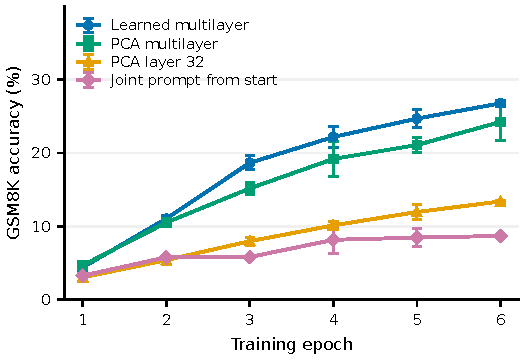
\includegraphics[width=.66\linewidth]{figures/representation_identity_sd.pdf}
\caption{\textbf{Identity-clock robustness.} The four models from Figure~\ref{fig:representationcomparison}, evaluated with $t=\tau$ and 32 steps. Points average seeds 42/123 and bars show $\pm1$ sample standard deviation across seed accuracies. Each epoch uses one trained checkpoint per arm.}
\label{fig:representationidentity}
\end{figure}

All four arms start from the same seed-42 ELF initialization, use 2,434,330 training rows, and preserve effective batch 512. The PCA multilayer run changes from two to four GPUs during training while maintaining that batch size. Each arm has one training run; seed variation in the figures measures sampling randomness only. The comparisons isolate projector choice at fixed layers and layer choice under PCA, without estimating their interaction. Paired intervals in the main text use 4,000 problem-bootstrap replicates and the four matched epoch-six generation seeds.
